% Power electronics---a controlled full-wave rectifier and
% it's output voltage and current waveforms.
% The delay angle \alpha is customizable. 
% Author: Ali Mehrizi-Sani
\documentclass[landscape]{article}
\usepackage[usenames,dvipsnames]{color}
\usepackage[american,cuteinductors,smartlabels]{circuitikz}
\usetikzlibrary{calc}
\ctikzset{bipoles/thickness=1}
\ctikzset{bipoles/length=0.8cm}
\ctikzset{bipoles/diode/height=.375}
\ctikzset{bipoles/diode/width=.3}
\ctikzset{tripoles/thyristor/height=.8}
\ctikzset{tripoles/thyristor/width=1}
\ctikzset{bipoles/vsourceam/height/.initial=.7}
\ctikzset{bipoles/vsourceam/width/.initial=.7}
\tikzstyle{every node}=[font=\small]
\tikzstyle{every path}=[line width=0.8pt,line cap=round,line join=round]

\definecolor{AleeRed}{rgb}{0.5,0,0}

\begin{document}
\begin{center}

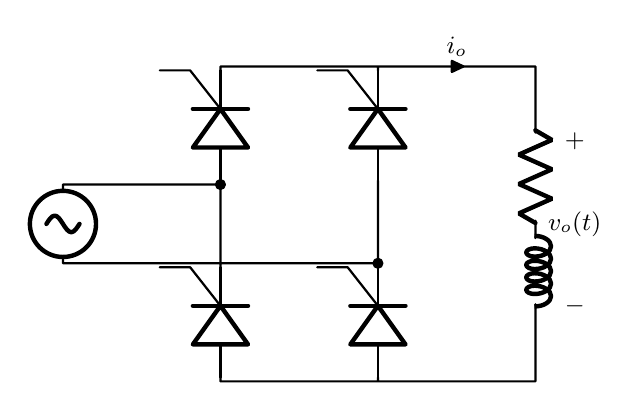
\begin{tikzpicture}
    \draw
    % Thyristors leg 2
    (2,0)
        to[Ty] ++(0,1.5)
        -- ++(0,1)
        to[Ty] ++(0,1.5) coordinate (leg2)
    % Thyristors leg 1
    (0,0)
        to[Ty] ++(0,1.5)
        -- ++(0,1)
        to[Ty] ++(0,1.5) coordinate (leg1)
    % Connections and load RL
        -- ++(2,0)
        to[short, i=$i_o$, current/distance=0.5] ++(2,0)
        -- ++(0,-0.8)
        to[R] ++(0,-1.2)
        to[L] ++(0,-1.2)
    % Back to (0,0)
        |- (0,0)
    % AC source
    (-2,1.5) coordinate (Vnn)
        to[sV] ++(0,1) coordinate (Vpp)
        -- (leg1 |- Vpp) node [circ] {}
    (Vnn)
        -- (leg2 |- Vnn) node [circ] {}
    % v_o(t)
    (4.5,3.5)
        to[open, v^=$v_o(t)$] ++(0,-3)
    ;
\end{tikzpicture}

\bigskip

% Example 4-7, p. 135 of Hart, discontinuous current in full-wave rect
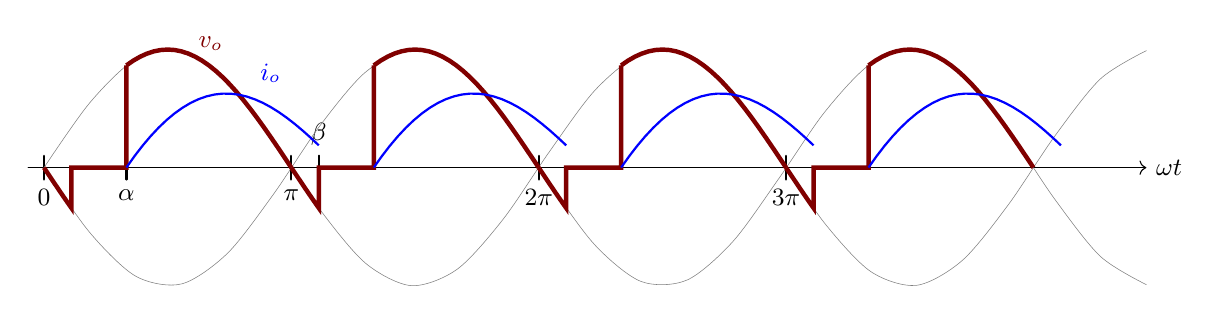
\begin{tikzpicture}
\begin{scope}[xscale=1,yscale=1.5]
    \newcommand{\alphaa}{60 * pi / 180}
    \newcommand{\betaa}{200 * pi / 180}

    \draw[thin, ->] (-0.2, 0) -- (14,0) node[right] {$\omega t$};

    \foreach \x/\xtext in {0,{\alphaa}/\alpha,{pi}/\pi,
      {\betaa}/~,{2*pi}/{2\pi},{3*pi}/{3\pi}}
        \draw (\x,0.1) -- (\x,-0.1) node [below] {$\xtext$};
    \draw (\betaa,-0.1) -- (\betaa,0.1) node [above] {$\beta$};


    % Vs
    \draw[domain=0:14, help lines, smooth]
        plot (\x,{sin(\x r)});
    % -Vs
    \draw[domain=0:14, help lines, smooth]
        plot (\x,{-sin(\x r)});
    % Vo and Io
    \foreach \qq [evaluate=\qq as \qqshft using \qq*pi] in {0,...,3}
    {
    \begin{scope}[xshift=\qqshft cm,
        every path/.style={ultra thick, color=AleeRed}]
        % Vo
         \draw[domain=0:{\betaa-pi}]
             plot (\x,{-sin(\x r)})
             -- ({\betaa-pi},0)
             -| (\alphaa,{sin(\alphaa r)})
         [domain=\alphaa:pi]
             plot (\x,{sin(\x r)});
         % Io
         \draw
         [domain=\alphaa:\betaa,color=blue,thick]
             plot (\x,{0.05 * (13.6*sin((\x - 0.646)*180/pi)
               - 21.2*exp(-\x/0.754))});
    \end{scope}
    }
    \node[right,color=AleeRed] at ({pi/2+pi/12},1.05) {$v_o$};
    \node[right,color=blue] at ({pi/2+pi/3},0.8) {$i_o$};
\end{scope}
\end{tikzpicture}

\end{center}
\end{document}